\documentclass{article}

% Language setting
% Replace `english' with e.g. `spanish' to change the document language
\usepackage[spanish]{babel}

% Set page size and margins
% Replace `letterpaper' with`a4paper' for UK/EU standard size
\usepackage[letterpaper,top=2cm,bottom=2cm,left=3cm,right=3cm,marginparwidth=1.75cm]{geometry}

% Useful packages
\usepackage{amsmath}
\usepackage{graphicx}
\usepackage[colorlinks=true, allcolors=blue]{hyperref}

\title{Parcial 2}
\author{Miguel Angel Alvarez, Jeisson Alvarez y Jackh Emmanuel Narvaez}

\begin{document}
\maketitle



\section{Análisis del problema}

empezamos abordando las posibles dificultades que se nos pueda ir presentando en el transcurso del trabajo iniciamos con la idea de poder hacer un codigo que pueda leer los pixeles que nos envien en la imagen jpg usando el poderoso Paint para la implementacion de nuestro ejemplo y asi ver como va leyendo la imagen o podríamos  


\section{Diseño}

\begin{figure}
\centering
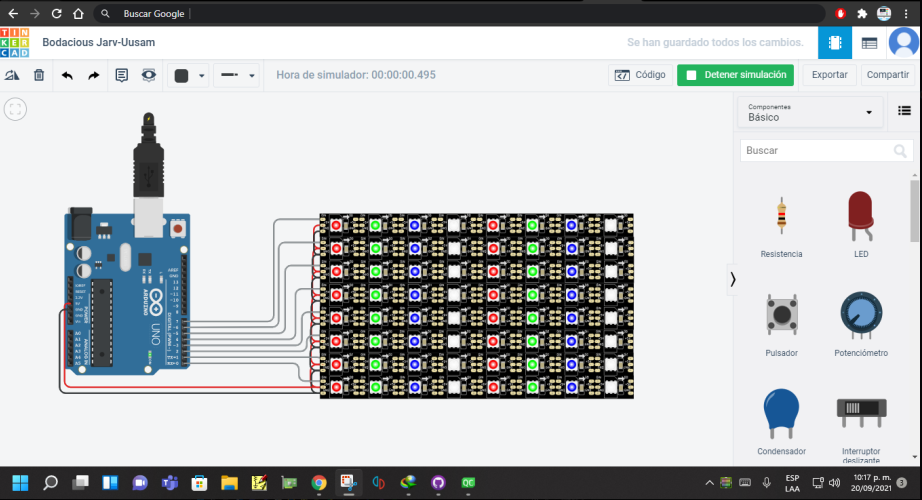
\includegraphics[width=0.5\textwidth]{image1.png}
\caption{diseño 1}
\end{figure}



\end{document}